\begin{flushleft}
	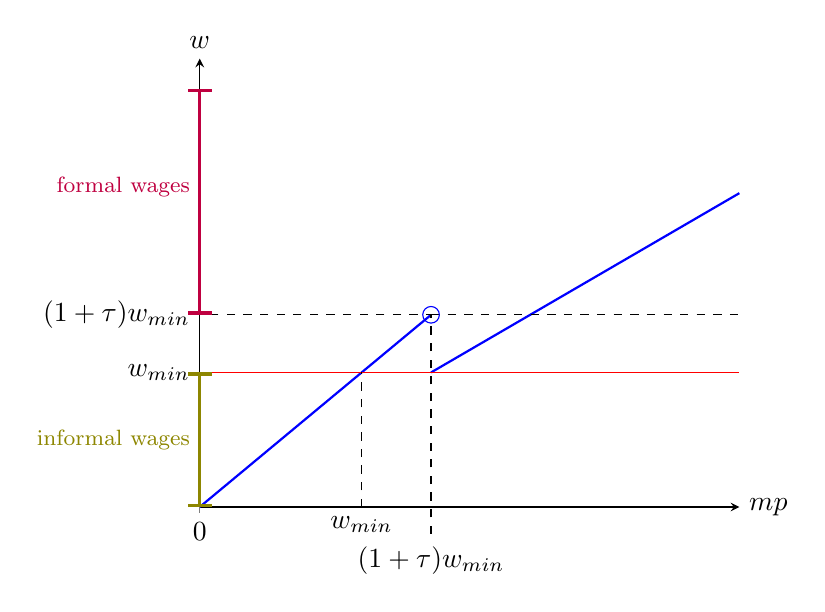
\begin{tikzpicture}
		\begin{axis}[
			% Insert parameters here
			scale=1,
			clip=false,
			xmin = 0, xmax = 15,
			ymin = 0, ymax = 15,
			axis lines = left,
			xtick = {0},
			ytick= \empty,
			]
			% Insert commands here
			% Labels of axes
			\node [right] at (current axis.right of origin) {$mp$};
			\node [above] at (current axis.above origin) {$w$};
			%\addplot[domain = 6.43:14, samples =
			%20, color = black, thick, dotted]{x};
			\addplot[domain = 0:6.43, samples =
			20, color = blue, thick]{x};
			\addplot[domain = 6.43:15, samples =
			20, color = blue, thick]{0.7*x};
			%\addplot[domain = 0:6.43, samples =
			%20, color = blue, thick, dotted]{0.7*x};
			\addplot[color = blue, mark=o, mark size=3pt]
			coordinates {(6.43, 6.43)};
			\addplot[domain = 0:15, samples =
			20, color = red, thin]{4.5};
			\node[left] at (0, 4.5) {$w_{min}$};
			\addplot[color = black, dashed]
			coordinates {(4.5, 0) (4.5, 4.5)};
			\node[below] at (4.5, 0) {$w_{min}$};
			\addplot[color = black, dashed]
			coordinates {(6.43, -0.9) (6.43, 6.43) (0, 6.43)};
			\node[below] at (6.43, -1) {$(1+\tau) w_{min}$};
			\node[left] at (0, 6.43) {$(1+\tau) w_{min}$};
			\addplot[color = black, dashed]
			coordinates {(6.43, 6.43) (15, 6.43)};
			%\draw [decorate,decoration={brace, amplitude=10pt, mirror, raise=4pt}, xshift=0cm, yshift=0pt, purple]
			%(14, 4.5) -- (14, 14.5) node [purple,midway,xshift=+1.5cm]
			%{\footnotesize formal wages};
			%\draw [decorate,decoration={brace, amplitude=10pt, mirror, raise=4pt}, xshift=0cm, yshift=0pt, olive]
			%(14, 0) -- (14, 6.43) node [olive,midway,xshift=+1.6cm]
			%{\footnotesize informal wages};
			\draw[|-|, olive, very thick] (0, 0) to (0, 4.5);
			\node[left, olive] at (0, 2.25) {\footnotesize informal wages};
			\draw[|-|, purple, very thick] (0, 6.43) to (0, 14);
			\node[left, purple] at (0, 10.71) {\footnotesize formal wages};
		\end{axis}
	\end{tikzpicture}
\end{flushleft}
